\documentclass[journal]{IEEEtran}
\usepackage[numbers]{natbib}
\usepackage{pgfplots}
\pgfplotsset{compat=1.18}
\usepackage{amsmath,amsfonts}
\usepackage{algorithmic}
\usepackage{array}
\usepackage{subcaption}
\usepackage{textcomp}
\usepackage{stfloats}
\usepackage{url}
\usepackage{verbatim}
\usepackage{booktabs}
\usepackage{multirow}
\usepackage{graphicx}
\usepackage{colortbl}
% \usepackage[table,xcdraw]{xcolor}
\usepackage{tikz}
\usepackage{titlesec}
\usepackage{authblk}
\usepackage{marvosym}
\usetikzlibrary{positioning, calc}
\usetikzlibrary{arrows}
\newcolumntype{P}[1]{>{\raggedright\arraybackslash}p{#1}}

\hyphenation{op-tical net-works semi-conduc-tor IEEE-Xplore}
% \def\BibTeX{{\rm B\kern-.05em{\sc i\kern-.025em b}\kern-.08em
    % T\kern-.1667em\lower.7ex\hbox{E}\kern-.125emX}}
\usepackage{balance}
\begin{document}
\title{bnmetamodel 2.0}

\author[1]{T. Griffiths\thanks{\textsuperscript{\Cross}Corresponding author: t.griffiths20@imperial.ac.uk}}
\author[2]{Z. Xuereb Conti}
\author[1]{M. Bluck}

\affil[1]{Department of Mechanical Engineering, Imperial College London, UK}
\affil[2]{Data-Centric Engineering / TRIC:DT, The Alan Turing Institute, UK}
\vspace{-15pt}

\maketitle

\begin{abstract}

\end{abstract}

\begin{IEEEkeywords}
Fusion power, metamodels, surrogate modelling, fusion commercialisation, machine learning, fusion economics, energy, Bayesian Networks
\end{IEEEkeywords}
\vspace{-2ex}

\section{Introduction}
Commercial-scale fusion power promises a future of reliable baseload, reduced carbon emissions, and enhanced energy security. Techno-economic modelling of future fusion power plants, faces challenges due to uncertain and imprecise costing models. To reason over uncertainty, efforts to estimate fusion power economics have been previously demonstrated using probabilistic methods[cite: Griffiths2024].

Despite these challenges, it is crucial for the fusion community to continue research efforts to predict both technical and economic performance metrics. The lack of such initiatives could hinder investment attraction, roadmap target achievement, and the promotion of additional investment opportunities. One way to address uncertainty is through the use of statistical methods, such as sensitivity analyses, during the modelling process. This allows decision-makers to evaluate key modelling variables more thoroughly and understand where improvements can be made to enhance the reliability of predictions.

Computational models offer a valuable tool for developing understanding in areas lacking experimental data. They provide the flexibility to simulate various scenarios and conditions rapidly, allowing for quick iteration and parameter modification. This enables swift exploration and optimisation of designs without the need for physical modifications or repeated experiments. Given the complexity of fusion engineering systems, computational models can effectively handle numerous variables and interactions, facilitating the analysis of large-scale systems with intricate behaviours.

This study extends the computational modelling technique applied in previous research to a new dataset, introducing enhancements and modifications to the method. The objective is to expand the application of Bayesian Networks (BNs) for a deeper understanding of fusion power design spaces, with a particular emphasis on economic aspects.


The study introduces an innovative approach to managing uncertainty in fusion research, diverging from traditional techniques. The surrogate modelling aims to create a more efficient model that replicates the output of a complex model, considering its inputs and parameters. In this context, a Bayesian Network acts as a surrogate for a fusion systems code [INSERT PyTOK REF?], predicting the economics of fusion power plants under uncertain data, with a specific focus on Spherical Tokamaks (STs).
This study builds on the surrogate modelling concept introduced by Griffiths et al. [cite: Griffiths2024], shifting the focus to a new case study. It employs data from a private fusion developer to reason about uncertain economic predictions of power plants. The integration of new data or information as additional nodes (either child or parent) is a key feature of this study, enhancing the model's inherent capacity to handle multiple outputs. The study delves deeper into validation methodologies and examines the influence of hyperparameters on the results. The application of soft evidence is also incorporated into the study. The findings of this research will provide valuable decision-making support for design spaces in fusion power.

The paper is structured as follows: Section~\ref{sec:background} provides a literature review of the topic, Section~\ref{sec:methodology} outlines the methodology, Section~\ref{sec:Results} presents the results, Section~\ref{sec:Discussion} discusses the results, and Section~\ref{sec:conc} concludes the paper. 

\section{Bayesian Networks}\label{sec:BNs}

Bayesian Networks (BNs) are a type of probabilistic graphical model that represents a set of variables and their conditional dependencies via a directed acyclic graph (DAG)~\cite{Hand2001IdiotsAll}. The nodes in the graph represent the variables, and the edges represent the dependencies between the variables. The conditional dependencies are represented by the edges between the nodes. The graph structure of a BN is a compact and intuitive way to represent the joint probability distribution of the variables. The joint probability distribution is the probability of each variable in the network taking on each of its possible states. The joint probability distribution can be factorised into a product of conditional probability distributions, one for each variable given its parents in the graph. This factorisation is known as the chain rule of probability.

The chain rule of probability, also known as the general product rule, allows the calculation of any member of the joint distribution of a set of random variables using only conditional probabilities.

Given a set of random variables, say $X_1, X_2, \ldots, X_n$, the chain rule of probability states that the joint probability of these variables is the product of the conditional probabilities of each variable given all the variables that precede it. Mathematically, this can be expressed as:

\begin{align}
    P(X_1, X_2, \ldots, X_n) = & P(X_1) \nonumber \\
    & * P(X_2 | X_1) \nonumber \\
    & * P(X_3 | X_1, X_2) \nonumber \\
    & * \ldots \nonumber \\
    & * P(X_n | X_1, X_2, \ldots, X_n-1)
    \label{eq:chain_rule}
\end{align}
    
In Equation \ref{eq:chain_rule}: $P(X1, X2, \ldots, Xn)$ is the joint probability of $X1$ through $Xn$. $P(X_i | X1, \ldots, X_i-1)$ is the conditional probability of $X_i$ given all the preceding variables.

Within the problem domain, each variable is represented by a node within the DAG, where the edges of the nodes serve to represent the relationship of one node to another. Koller and Friedman explain that these DAGs can be interpreted as: \textit{a data structure, which acts as the foundational framework for efficiently representing the joint distribution in a factorised manner}. Each node in the graph represents a variable, and the directed edges indicate conditional dependencies between two variables. The parameters of a BN specify the conditional probabilities associated with each node given its parents in the network. Parameters in a BN are associated with the conditional probability distributions (CPDs) of the network's variables. A BN consists of nodes representing variables and edges representing dependencies between variables. The parameters of a BN specify the conditional probabilities associated with each node given its parents in the network. These conditional probabilities determine the relationships and dependencies between variables in the BN. By using a BN, it is not necessary to explicitly specify all the parameters of the joint probability distribution (JPD). The joint probability distribution can be factorised into a product of conditional probability distributions, one for each variable given its parents in the graph. This factorisation is known as the chain rule of probability. The structure of the BN captures the dependencies between variables, and the conditional probabilities are derived from data or expert knowledge. This allows for efficient representation of the JPD without explicitly specifying all the individual parameters, making BNs a powerful tool for probabilistic modelling. When multiple probability distributions are combined, a Joint Probability Distribution (JPD) is formed. These represent the probability of every possible combination of values of each variable. Consequently, when combined, a BN forms a structure of interdependent variables that efficiently represents a JPD without the need to explicitly specify all the parameters. This provides a compact representation by combining the \textit{local} conditional distributions for each node, with respect to its connected parent nodes~\cite{Koller2009ProbabilisticTechniques}, see Figure~\ref{fig:BN3}.

\begin{figure}[ht]
    \centering
    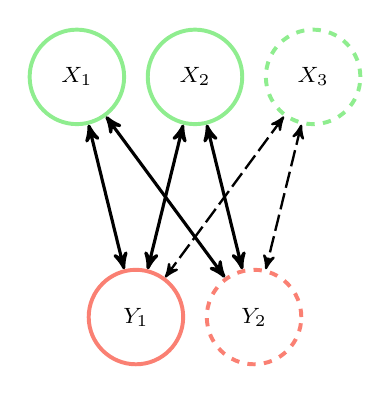
\begin{tikzpicture}[node distance=1.5cm, font=\footnotesize, align=center, >=stealth', line width=0.5mm]
        % Define colors
        \definecolor{lightgreen}{rgb}{0.56, 0.93, 0.56}
        \definecolor{lightred}{rgb}{0.98, 0.5, 0.45}

        % Nodes
        \node[draw, circle, draw=lightgreen, text=black, minimum size=1.2cm] (input1) {$X_1$};
        \node[draw, circle, draw=lightgreen, text=black, right of=input1, minimum size=1.2cm] (input2) {$X_2$};
        \node[draw, circle, dashed, draw=lightgreen, text=black, right of=input2, minimum size=1.2cm] (input3) {$X_3$};

        \node[draw, circle, draw=lightred, text=black, below=1.8cm of input2, xshift=-0.75cm, minimum size=1.2cm] (output1) {$Y_1$};
        \node[draw, circle, dashed, draw=lightred, text=black, below=1.8cm of input2, xshift=0.75cm, minimum size=1.2cm] (output2) {$Y_2$};

        % Edges
        \foreach \i in {1,...,2} {
            \foreach \j in {1,...,2} {
                \draw[<->, line width=0.4mm] (input\i) -- (output\j);  % Decreased line width
            }
        }
        \foreach \j in {1,...,2} {
            \draw[<->, dashed, dash pattern=on 6pt off 2pt, line width=0.3mm] (input3) -- (output\j);  % Decreased line width and less 'dashed'
        }
    \end{tikzpicture}
    \caption{\small Graphical representation of Bayesian Network where nodes $X_i$ represent the input variables and the nodes $Y_i$ represent the output variables to the analytical model. The solid lines represent the existing nodes in the model. Dashed line nodes representing those that are not present in the original model but can be added to the model as part of adapting the engineering environment as new information is gathered.}\label{fig:BN3} 
    \vspace{-15pt}
\end{figure}

In depth, the term \textit{prior} refers to the initial probability distribution assigned to a variable. On the other hand, the \textit{posterior} probability refers to the updated probability distribution after \textit{prior} beliefs are updated via \textit{inference}, based on available evidence. The primary benefit of a probabilistic representation lies in its ability to perform \textit{probabilistic inference}, which enables bi-directional reasoning with uncertain information using probabilistic methods. Thus, adopting a BN as a surrogate model facilitates exploration of causal relationships between fusion parameters and cost in both forward and reverse directions, allowing for an uncertain fusion parameter design space to be mapped from a desired cost. 

By defining inference as the process of making deductions based on evidence, reasoning and, prior knowledge, it is possible to further characterise Bayesian inference as the act of making alterations to existing probability distributions to discover how, based on their causal relationships, the variable's remaining probability distributions are altered. This acts as a useful tool to measure and understand relationships between inputs and responses in engineering design spaces~ \cite{Koller2009ProbabilisticTechniques}. One limitation of BNs is their inability to handle continuous data. However, real-world data often comprises a mixture of discrete and continuous variables. While some implementations of BNs with continuous data have been proposed~\cite{Cobb2007BayesianVariables,Chen2017LearningData, Li2018EfficientVariables}, data used to configure a BN requires a discretisation process. Refer to Section~\ref{sec:design} for an overview of the discretisation method used in this study.

\subsection{Literature review}~\label{sec:background}

Include your own work from previous paper and include work from Pavonne et al 2023. 

\section{Methodology}\label{sec:methodology}

\begin{figure*}[t]
    \centering
    \includegraphics[width=\textwidth]{figures/workflow_v3.png}
    \caption{Workflow of the surrogate modelling process.}\label{fig:workflow}
\end{figure*}

In this section, steps are outlined for the creation, application of a Bayesian Network (BN) as a surrogate model. Adapated from Conti 2019 and Griffiths 2024, Figure~\ref{fig:workflow} delineates a step-wise algorithm for the creation, cross-validation, and application of BN as a surrogate model. 

[Link the steps in the figure to the text below. Then add another section that delininates what was done in this study using specifics, i.e., what data was used, what model was used, what was the output, etc.]

\subsection{Define design variables}\label{sec:design}
This step involves making a strategic decision on which component or system will be the focus of the model. For instance, we might choose to model a whole reactor system, or a critical component like the breeder blanket or the divertor. The chosen component's key parameters and characteristics are then defined as input variables, denoted as $X_1$, $X_2$,\ldots, $X_n$..

Ahead of executing the selected analytical model, it requires configuration. This process includes choosing the inputs and outputs, along with defining the value ranges for each variable. The selection of inputs and outputs is guided by the objectives of the analysis and the data at hand. The value ranges for each variable are set considering the system's physical limitations and the required granularity of the analysis. Once configured, the analytical model is run to produce the dataset, which is then utilised to set up the Bayesian Network (BN). Typically, BNs perform better at making predictions when the input distribution is uniform. This is for several reasons: Model assumptions: normal distributions assume a bell-shaped curve with values concentrated around a mean, while uniform distributions make no assumptions about data shape and better capture the true underlying distribution. Nonlinearity and Outliers: normal distributions are sensitive to outliers, as they can significantly impact the mean and standard deviation, which may not accurately represent the underlying relationship between variables. Uniform distributions, being less influenced by extreme values, can provide a more robust representation of the data. Flexibility and Non-parametric Modelling: Uniform distributions offer flexibility in modelling unknown or non-normally distributed data without relying on specific distribution assumptions, allowing the BN to adapt and capture complex relationships. Simplification of Model Complexity: Normal distributions require additional parameters (mean and standard deviation) that necessitate estimation, increasing model complexity and the number of parameters to learn. In contrast, using uniform distributions simplifies the model by eliminating the need for extra parameter estimation, resulting in easier training and interpretation~\cite{Duda1973PatternAnalysis, Neapolitan2004LearningNetworks, Koller2009ProbabilisticTechniques}.

\subsection{Deterministic model}\label{sec:deterministic}
This is the model that is replicated by the BN. It should be noted that the deterministic model is not limited to a single model, but can be a combination of models. It should have the capability to provide the output variables, denoted as $Y_1$, $Y_2$,\ldots, $Y_m$, and collect data for the surrogate model. 

\subsection{Parameter Selection}\label{sec:parameters} This step involves identifying and selecting the input parameters for the surrogate model that significantly influence the output being modeled.

\subsection{Data Collection and Parameter Estimation}\label{sec:data} The deterministic model is run at this stage to gather data that will be used to configure the surrogate model. It's crucial to collect data that represents the entire design space to ensure the accuracy of the surrogate model. Therefore, specific sampling techniques, such as Latin Hypercube or Sobol sampling, are used to ensure that the data collected is representative of the entire design space.

\subsection{Bayesian Network Configuration}\label{sec:BNconfiguration}

The Bayesian Network is configured at this stage to mirror the deterministic model, using the inputs selected in step~\ref{sec:parameters} and the data collected in step~\ref{sec:data}. The data is discretised either by equidistant binning or by percentiles, for inputs and outputs respectively.

BNs are designed to handle discrete distributions, which means that datasets need to be discretised into bins before they can be used. This discretisation process is necessary to convert continuous data into discrete categories or intervals that the BN can handle effectively. This corresponds to Step 2 in Figure~\ref{fig:workflow}. By discretising the dataset into appropriate bins, the BN can leverage the discrete nature of the variables and make probabilistic inferences. Discretisation is a method used in machine learning to transform continuous variables into discrete categories or bins. For this study, two distinct methods of discretisation are employed: \textit{equal distance} and \textit{percentile binning}. For the inputs, the \textit{equal distance} approach was applied, while the \textit{percentile binning} method was implemented for the target, i.e., capital cost. This differentiation allows for an effective and tailored discretisation process that accommodates the specific characteristics and requirements of the inputs and outputs.

Equal distance binning divides the range of a variable into a fixed number of equal-sized intervals or bins. This method assigns values to bins based on their proximity to the bin boundaries. Equal distance binning is commonly used for discretising input features in machine learning because it preserves the linear relationship between the variable values and allows for easy interpretation of the results. It can be particularly useful when the variable exhibits a linear trend or when the absolute values of the variable are important for the prediction task, making it the most appropriate method during the initial construction of the BN. 

On the other hand, percentile binning divides the data based on the distribution of the variable values. Each bin contains an equal number or percentage of data points, ensuring that the bins capture an approximately equal amount of information. Percentile binning is often preferred for discretising target or output variables in ML. This is because output data distributions are typically less uniform. It can thus help handle class imbalance issues, i.e., bias, and create more balanced categories for classification tasks. By grouping data points based on their relative positions in the distribution, percentile binning can ensure that each bin represents a similar portion of the target variable, reducing the impact of outliers and enhancing model performance. Overall, the selection of the appropriate discretisation method should be based on an understanding of the data distribution, the specific machine learning task, and the goals of the analysis. 

Once discretised into probability distributions, both inputs and outputs from training data configure the BN, corresponding to Step 3 in Figure~\ref{fig:workflow}. In this step, the BN learns the parameters and develops the causal relationships between them, i.e., populates the conditional probability tables with the prior distributions of the variables. 

In this context, the pre-configured and validated BN is employed to perform bi-directional inference. Forward inference involves updating prior assumptions of inputs, utilising available evidence to give the output response. Conversely, reverse inference involves estimating the inputs given the output. The ability to perform reverse inference stems from the fact that once a BN has learned the parameters, it no longer differentiates between inputs and outputs. This characteristic allows the network to infer in both directions, making it possible to predict inputs based on output data. This step corresponds to Step 5 in Figure~\ref{fig:workflow}.

\subsection{Model Validation and Testing}\label{sec:meth_validation} 

Next, input testing data (excluding the outputs) is used to begin validation, which measures model accuracy. As part of the validation procedure and in order to avoid bias, a partitioning technique was used to partition the dataset into training and testing in $k$ distinct manners, known as $k$-fold cross-validation. This means the BN was built, and then validated $k$ times, with $k$ unique combinations of training and $k$ testing sets. The ratio of the split between training and testing sets in each fold is determined by the number of folds used to split the dataset by $1/k$, e.g., 3 folds will have a test split size of $1/3 = 33\%$. The validation itself corresponds to Step 4 in Figure~\ref{fig:workflow}, however the dataset is split after discretisation (Step 2), and ahead of BN configuration (Step 3). 

In order to quantify how well the model makes predictions compared to the analytical response, the predicted values were compared with the actual values in the testing data. In traditional machine learning evaluation methods like Root Mean Square Error (RMSE), the predictions and actual values are typically scalar values, such as numerical measurements or continuous variables. However, in the context of BNs, the outputs are probabilistic, distributions, or categorical variables rather than single numerical values. As a result, standard evaluation metrics like RMSE are not directly applicable, and alternative or custom approaches must be used to assess the performance of BN models. This can done either by (i) calculating the difference between the mean of the predicted bin and the simulated value in the testing data, $d_{1}$, (ii) calculating the difference between the mean of the predicted bin and the mean of the bin in which the actual simulated value lies, $d_{2}$. See [FIG].

The NDE is a measure used to assess the relative magnitude of the distance error in relation to the range of values in a given bin. It helps to put the distance error into perspective and make it comparable across different bin ranges. By dividing the distance error by the difference between the maximum and minimum bin range values, a normalised distance error is obtained that takes into account the scale and range of the data. This normalisation allows for a fair comparison of the distance error across different bin ranges, providing a standardised measure of the error~\cite{Conti2019BayesianDesign}. See~\ref{sec:res_validation}. 

\section{Results}\label{sec:Results} 

Section~\ref{sec:res_validation} provides an overview of the outcomes obtained through $k$-fold cross-validation. Section~\ref{sec:res_forward} presents the findings from forward inference with the BN, focusing on the prediction of capital cost ranges concerning uncertain, yet economically significant, fusion input parameters. In contrast, Section~\ref{sec:res_reverse} delves into the outcomes of reverse inference with the BN, emphasising the prediction of ranges for economic fusion parameters while considering uncertainties in capital cost. Lastly, Section~\ref{sec:res_decision} offers insights from hybrid evidence analyses, wherein both capital cost and specific fusion economic input parameters are constrained through choice observational evidence. These analyses aim to predict the remaining unfixed fusion economic input parameters under conditions of uncertainty.

\subsection{Validation of the Bayesian Network}\label{sec:res_validation}
To enable $k$-fold cross-validation, the dataset was split into 10 folds. 10 fold cross-validation aligns with the recommendation by Marcot et al.~\cite{Marcot2021WhatAnalysis}, who support the prevalent use of $k$=10 for Bayesian networks in literature. Plotting the NDE in a histogram provides a good illustration of model performance, see Figure~\ref{fig:k-foldhistograms}. The resulting validation plot distributions in~\ref{fig:k-foldhistograms} provide an intuitive indication of how well the BN predicts the numerical responses. Overall, when observing the distribution of the d1 plots for all 10 folds, it can be noted that the BNM built on 10,000 data points, seems to predict the correct response with an average 94.79\% accuracy.

\begin{figure*}
    \centering
    \includegraphics[width=0.9\textwidth]{figures/st20_d1_7bins_folds.png}
    \caption{\small Normalised probability histograms with prediction accuracy values for the first fold is shown for $d_{1}$ bin resolution = 7, dataset size = 10240.}
    \label{fig:k-foldhistograms}
\end{figure*}

\subsection{Hyperparameter Tuning}\label{sec:res_hyperparameter}
Using the data, calibration of hyper-parameters (such as bin resolution and dataset sizes) were examined by exploring two factors: (i) utilising three distinct dataset sizes and, (ii) experimenting with different bin resolutions during discretisation. The objective was to determine appropriate values for each factor and optimise the BN accordingly. Consequently, for (i) this meant dataset sizes of 1400, 5120, and 10240 and, for (ii), changing the number of bins between, 5, 7 and 10, respectively. The findings of this study are presented in [FIG], illustrating that the model exhibited optimal performance when applying the largest dataset and employing a bin resolution of 7. In general, the average prediction accuracy for $d_{2}$ errors tends to be higher than that for $d_{1}$ errors, except in the case of using high bin resolutions.

\begin{figure*}[h]
    \centering
    \includegraphics[width=0.6\textwidth]{figures/SA_3D_trimmed_39.png}
    \caption{\small A grouped bar chart displaying the average accuracy of predictions for $d_{1}$ and $d_{2}$ errors while investigating variations in both (i) the size of the dataset and (ii) the resolution of bins.}~\label{fig:3D_SA_trimmed_39_D1}
\end{figure*}

\subsection{Forward Inference}\label{sec:res_forward}

\subsection{Reverse Inference}\label{sec:res_reverse}

Addition of new data or information will be included. Addition of new node (child or parent) will be included. Addition of soft evidence will be included.

\subsection{Case Study: Component Decision Support}\label{sec:res_decision} 
Results from the model provide decision support for components, such as determining input ranges for optimal performance based on a desired output using reverse inference.

For~\ref{sec:design}, the system modelled was a whole reactor. The purpose was to determine how important output parameters vary with certain inputs. For~\ref{sec:deterministic} the deterministic  model used was `PyTOK', a Tokamak Energy systems code that finds optimum working point using a series of 0D and 1D approximations that model all subsystems. Previous studies from Griffiths et al. 2024 have shown that PROCESS is a suitable model for this purpose. For~\ref{sec:parameters}, the important parameters were selected from the PyTOK model, for inputs, these were: major radius, aspect ratio, effective ion charge, and toroidal field on plasma. For the outputs, these were: $Q_{\text{engineering}}$, high grade wasteheat, net electrical output, and capital cost. For~\ref{sec:data}, The input space was sampled between the parameter limits using Saltelli's extension of the Sobol sequence [CITATIONS], a quasi-random low-discrepancy sequence used to generate pseudo-uniform samples of parameter space. Data was collected from the PyTOK model to produce a dataset size of 10,000. For~\ref{sec:BNconfiguration}, the Bayesian Network was configured to replicate the deterministic model using the inputs outlined in above for~\ref{sec:parameters}, see Figure~\ref{fig:BN2}. For~\ref{sec:meth_validation}, the model was validated using $k$-fold cross-validation. For~\ref{sec:res_decision}, the model was used to provide component decision support.

\begin{figure}[h]
    \centering
    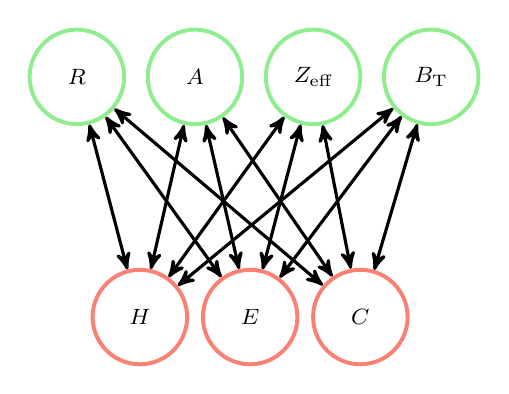
\begin{tikzpicture}[node distance=1.5cm, font=\footnotesize, align=center, >=stealth', line width=0.5mm]
        % Define colors
        \definecolor{lightgreen}{rgb}{0.56, 0.93, 0.56}
        \definecolor{lightred}{rgb}{0.98, 0.5, 0.45}

        % Nodes
        \node[draw, circle, draw=lightgreen, text=black, minimum size=1.2cm] (input1) {$R$};
        \node[draw, circle, draw=lightgreen, text=black, right of=input1, minimum size=1.2cm] (input2) {$A$};
        \node[draw, circle, draw=lightgreen, text=black, right of=input2, minimum size=1.2cm] (input3) {$Z_{\text{eff}}$};
        \node[draw, circle, draw=lightgreen, text=black, right of=input3, minimum size=1.2cm] (input4) {$B_{\text{T}}$};

        \node[draw, circle, draw=lightred, text=black, below=1.8cm of input2, xshift=-0.7cm, minimum size=1.2cm] (output2) {$H$};
        \node[draw, circle, draw=lightred, text=black, below=1.8cm of input2, xshift=0.7cm, minimum size=1.2cm] (output3) {$E$};
        \node[draw, circle, draw=lightred, text=black, below=1.8cm of input2, xshift=2.1cm, minimum size=1.2cm] (output4) {$C$};

        % Edges
        \foreach \i in {1,...,4} {
            \foreach \j in {2,...,4} {
                \draw[<->, line width=0.4mm] (input\i) -- (output\j);  % Decreased line width
            }
        }
    \end{tikzpicture}
    \caption{\small Graphical representation of Bayesian Network where nodes represent the input variables (Major Radius $R$, Aspect Ratio $A$, Effective Ion Charge $Z_{\text{eff}}$, Toroidal Field on Plasma $B_{\text{T}}$) and the output variables (High Grade Wasteheat $H$, Net Electrical Output $E$, Capital Cost $C$) to the analytical model.}\label{fig:BN2} 
    \vspace{-15pt}
\end{figure}

\begin{figure*}[h]
    \centering
    \includegraphics[width=0.9\textwidth]{figures/newplotting_test.png}
    \caption{Resulting posterior output distributions (red) for reverse
    inference on the selected input bins (green).}\label{fig:results}
\end{figure*}

\section{Discussion}\label{sec:Discussion}

\subsection{Validation of the Bayesian Network}\label{sec:disc_validation}

\subsection{Hyperparameter Tuning}\label{sec:disc_hyperparameter}

\subsection{Forward Inference}\label{sec:disc_forward}

\subsection{Reverse Inference}\label{sec:disc_reverse}

\section{Conclusion and Further Work}\label{sec:conc}

\section{Acknowledgments}
This research was supported by the EPSRC (Engineering and Physical Sciences Research Council, UK) Nuclear Energy Futures Centre for Doctoral. Training in Nuclear Energy (NEF CDT).  Other research studies under the NEF CDT involving Thomas Griffiths are supported in part by Tokamak Energy Ltd, UK. Views and opinions expressed are however those of the author(s) only a do not nsolidloosely dottedecessarily reflect those of Tokamak Energy Ltd.

\bibliographystyle{plainnat}
\bibliography{References}

\end{document}